\section{Étude de l'action de préhension \label{sec_5}}

\begin{obj}
L'objectif de cette partie est de valider les performances de serrage de la pince et de vérifier
les critères suivants du cahier des charges.
\begin{center}
\begin{tabular}{ll}
\hline
\textbf{Critère} & \textbf{Valeur} \\ \hline \hline
Diamètre des objets à saisir entre & \SI{40}{mm} et \SI{300}{mm} \\ 
Masse maximale des objets à saisir & \SI{2,5}{kg} \\
\hline
\end{tabular}
\end{center}
\end{obj}


\subsection{Actions mécaniques dans la pince}

\begin{obj}
Dans cette sous-partie, on établit la transmission des actions mécaniques entre
l'actionneur et l'effecteur et on quantifie les actions à fournir par l'actionneur pour respecter
le cahier des charges.
\end{obj}


\ifprof
\else

La pince de préhension, servant à collecter les échantillons de roche ou à poser/prendre des
instruments sur le sol, est une pince à trois doigts (préhenseur tridigital, voir \autoref{fig_23}). Par
symétrie, on restreint l'étude à un seul doigt.
La chaîne cinématique correspondante est schématisée (modélisation plane) sur la \autoref{fig_23} ; elle
est constituée :
\begin{itemize}
\item du bâti 0 lié au bras manipulateur du système ROBOVOLC, auquel on associe le repère $\left(P,\vect{x_P},\vect{y_P},\vect{z_P}\right)$ avec
$\vect{x_P}$ la verticale descendante ;
\item  d'un vérin 1 en liaison glissière de direction $\vect{x_P}$ avec le bâti 0 ;
\item  d'une tige 2 en liaison pivot d'axe $\left(H,\vect{z_P}\right)$ avec le vérin 1 ;
\item  de deux biellettes 3 et 4 parallèles et en liaisons pivot d'axes respectifs $\left(A,\vect{z_P}\right)$ et $\left(C,\vect{z_P}\right)$
avec le bâti 0. La biellette 3 est également en liaison pivot d'axe $\left(E,\vect{z_P}\right)$ avec la tige 2 ;
\item  d'un mors 5 en liaisons pivot d'axes $\left(B,\vect{z_P}\right)$ et $\left(D,\vect{z_P}\right)$ avec les biellettes 3 et 4 ;
\item  d'un galet 6 en liaison rotule de centre $Q$ avec le mors 5 et en contact avec l'objet à saisir.
\end{itemize}
Les points $A$, $B$, $C$, $D$ forment un parallélogramme. On introduit le paramétrage suivant :
$d=\vect{HP} \cdot \vect{y_P}=\vect{AP} \cdot \vect{y_P}=\vect{CP} \cdot \vect{y_P}$, 
$CE = EH = \ell_2$, 
$AC = BD = \ell_3$,
$AB = CD = \ell_4$,
$\vect{DQ} = L_5\vect{x_P} + \ell_5 \vect{y_P}$, 
$\vect{QS} = \ell_6\vect{y_P}$
ainsi que les angles
$\alpha = \left(\vect{HC},\vect{HE}\right)$
et  $\beta = \left(\vect{y_P},\vect{EC}\right)$.

On donne $d = \SI{50}{mm}$, $\ell_2 =\SI{100}{mm}$, $\ell_4 =\SI{150}{mm}$, $\ell_5 =\SI{20}{mm}$, $\ell_6 =\SI{15}{mm}$.

\begin{figure}[H]
\centering
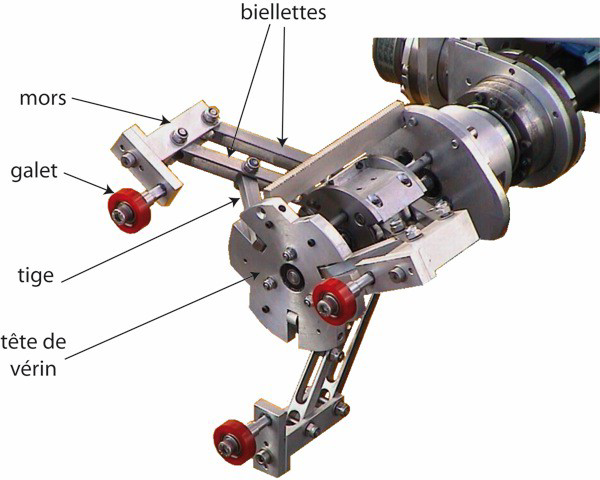
\includegraphics[width=.45\linewidth]{fig_23a.png}
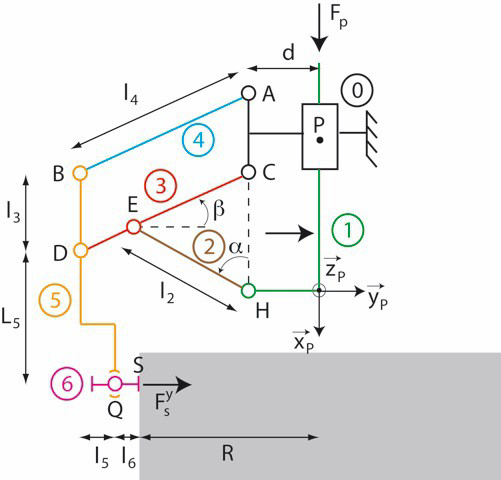
\includegraphics[width=.45\linewidth]{fig_23b.png}
\caption{Pince utilisée sur le système ROBOVOLC et schéma cinématique associé \label{fig_23}}
\end{figure}


Le contact entre le galet 6 et l'objet est modélisé par une liaison linéaire rectiligne d'axe $\left(S,\vect{x_P}\right)$ et
de normale $\vect{y_P}$ .
Dans une première approche, on considère que toutes les liaisons sont parfaites. De plus, le poids
des pièces composant la pince est négligé.
L'objet à saisir est modélisé par un cylindre à base circulaire de rayon $R$.
\fi


% QUESTION SUPPLEMENTAIRE
\question{Dans cette question uniquement, on considère le système formé par les pièces 0, 3, 4 et 5. Déterminer degré d'hyperstatisme du modèle. S'il est hyperstatique, proposer une ou plusieurs modifications de liaisons pour le rendre isostatique.}
\ifprof
\begin{corrige}
Dans cette configuration on a : 
\begin{itemize}
\item $m=1$ : mobilité du parallélogramme;
\item $E_S = 6\times 3 = 18$;
\item $I_S = 4\times 5 = 20$ : 4 laisons pivot.
\end{itemize}
Au final : $h=m-E_S+I_S = 1 -18+20 = 3$.
Il suffit de remplacer une liaison pivot par une liaison sphère-cylindre.

\end{corrige}
\else
\fi

% QUESTION SUPPLEMENTAIRE
\question{Tracer le graphe de liaisons. Déterminer degré d'hyperstatisme du modèle complet.}
\ifprof
\begin{corrige}
\begin{itemize}
\item $m=2$ : mobilité du parallélogramme commandé et du galet 6 (rotation propre);
\item $E_S = 6\times 6 = 36$;
\item $I_S = 6\times 5 + 1\times 6  + 3 + 2=41$ : 6 laisons pivot, 1 glissière, 1 rotule, 1 cylindre plan.
\end{itemize}
Au final : $h=m-E_S+I_S = 2 -36+41 = 7$.

\end{corrige}
\else
\fi


% Q5.1
\question{Donner le lien entre les angles $\alpha$ et $\beta$, ainsi que l'expression de ces angles en fonction du
rayon $R$ de l'objet et des données géométriques.}
\ifprof
\begin{corrige}
Une fermeture géométrique angulaire dans le triangle $CEH$ donne immédiatement :  $\alpha + \beta =\dfrac{\pi}{2}$.

Une fermeture géométrique linéaire permet de déterminer la relation entre  $\alpha$ (ou $\beta$), $R$ et les dimensions du mécanisme.
On trouve (en projetant sur l’axe $\vect{x}$) :
$\left\{
\begin{array}{l}
R = d + l_4 \cos\beta -l_5 - l_6 \\
R = d + l_4 \sin\beta -l_5 - l_6 \\
\end{array}
\right.
$.

\end{corrige}
\else
\fi

% Q5.2
\question{Montrer que la liaison équivalente entre le mors 5 et l'objet à saisir est une liaison ponctulle de normale $\left(S,\vect{y_P}\right)$. Cette liaison équivalente
sera utilisée dans la suite de cette partie.}
\ifprof
\begin{corrige}
Les liaisons étant en série, il est plus direct de passer par les torseurs cinématiques. Nous avons ici l’association d’une liaison rotule et d’une liaison appui plan en série
$\torseurcin{V}{5}{\text{objet}} = \torseurcin{V}{5}{6} + \torseurcin{V}{6}{\text{objet}}$.

$\torseurcin{V}{5}{\text{objet}} 
= 
\torseurl{\omega_{x56} \vect{x_P}+\omega_{y56} \vect{y_P}+\omega_{z56} \vect{z_P}}
{\vect{0}}{Q}
+ \torseurl{\omega_{y60} \vect{y_P}}{V_x \vect{x_P}+V_z \vect{z_P}}{Q}
= 
\torseurl{\omega_{x} \vect{x_P}+\omega_{y} \vect{y_P}+\omega_{z} \vect{z_P}}
{V_x \vect{x_P}+V_z \vect{z_P}}{Q}
$.

Il s’agit du torseur d’une liaison ponctuelle de normale $(Q,\vect{y_P})$,  la forme du torseur est maintenue sur la droite $(Q,\vect{y_P})$, la liaison peut donc s’exprimer également comme une ponctuelle de normale  $(S,\vect{y_P})$.

\end{corrige}
\else
\fi

% Q5.3
%\question{Calculer l'hyperstatisme du modèle plan du mécanisme global de la pince (\autoref{fig_23}).}

% Q5.4
\question{Donner l'orientation de l'effort dans les liaisons pivot situées en $B$ et en $E$.}
\ifprof
\begin{corrige}
Les solides 2 et 4 sont soumis chacun à 2 glisseurs, par conséquent, les directions des efforts  en $B$ et $E$ sont respectivement $\vect{AB}$ et $\vect{EH}$.
\end{corrige}
\else
\fi

\ifprof\else
L'ouverture/fermeture de la pince est réalisée par un moteur électrique et un système vis-écrou
fournissant un effort de poussée $\vect{F_P}=F_p\vect{x_P}$ sur le vérin 1 en amont de la pince. D'autre part, on
introduit à présent un modèle de frottement au contact entre le galet 6 et l'objet à saisir. Ce modèle
se traduit au niveau de la liaison équivalente entre le mors 5 et l'objet à saisir par un torseur
statique de la forme : $\torseurstat{T}{5}{\text{objet}}=\torseurl{-F_S^x\vect{x_P}+F_S^y\vect{y_P}}{\vect{0}}{S}$ 
où $F_S^x$ est l'effort tangentiel et $F_S^y$ est l'effort normal (ou de serrage) au contact.
\fi

%% Q5.5
%\question{Par une étude statique, montrer que les efforts $F_P$, $F_S^x$ et $F_S^y$ 
%y sont liés par la relation $F_P = K \left( \tan \beta F_S^y - F_S^x\right)$  
%où l'expression de la constante $K$ est à préciser en fonction de $\ell_2$ et $\ell_4$.
%Montrer également que cette relation est indépendante de la longueur $L_5$ et expliquer l'avantage technique de ce résultat. }

% Question modifiiée
\question{Par une étude statique, on peut montrer que les efforts $F_P$, $F_S^x$ et $F_S^y$ sont liés par la relation $F_P = K \left( \tan \beta F_S^y - F_S^x\right)$  
où l'expression la constante $K$ s'exprime en fonction de $\ell_2$ et $\ell_4$.
Proposer une stratégie (isolement, théorèmes utilisé, point d'application si nécessaire, projection) permettant d'établir cette relation. On s'appuiera sur le graphe de liaison établiu précédemment.}
%Montrer également que cette relation est indépendante de la longueur $L_5$ et expliquer l'avantage technique de ce résultat. }

\ifprof
\begin{corrige}~\\
\begin{figure}[H]
\centering
{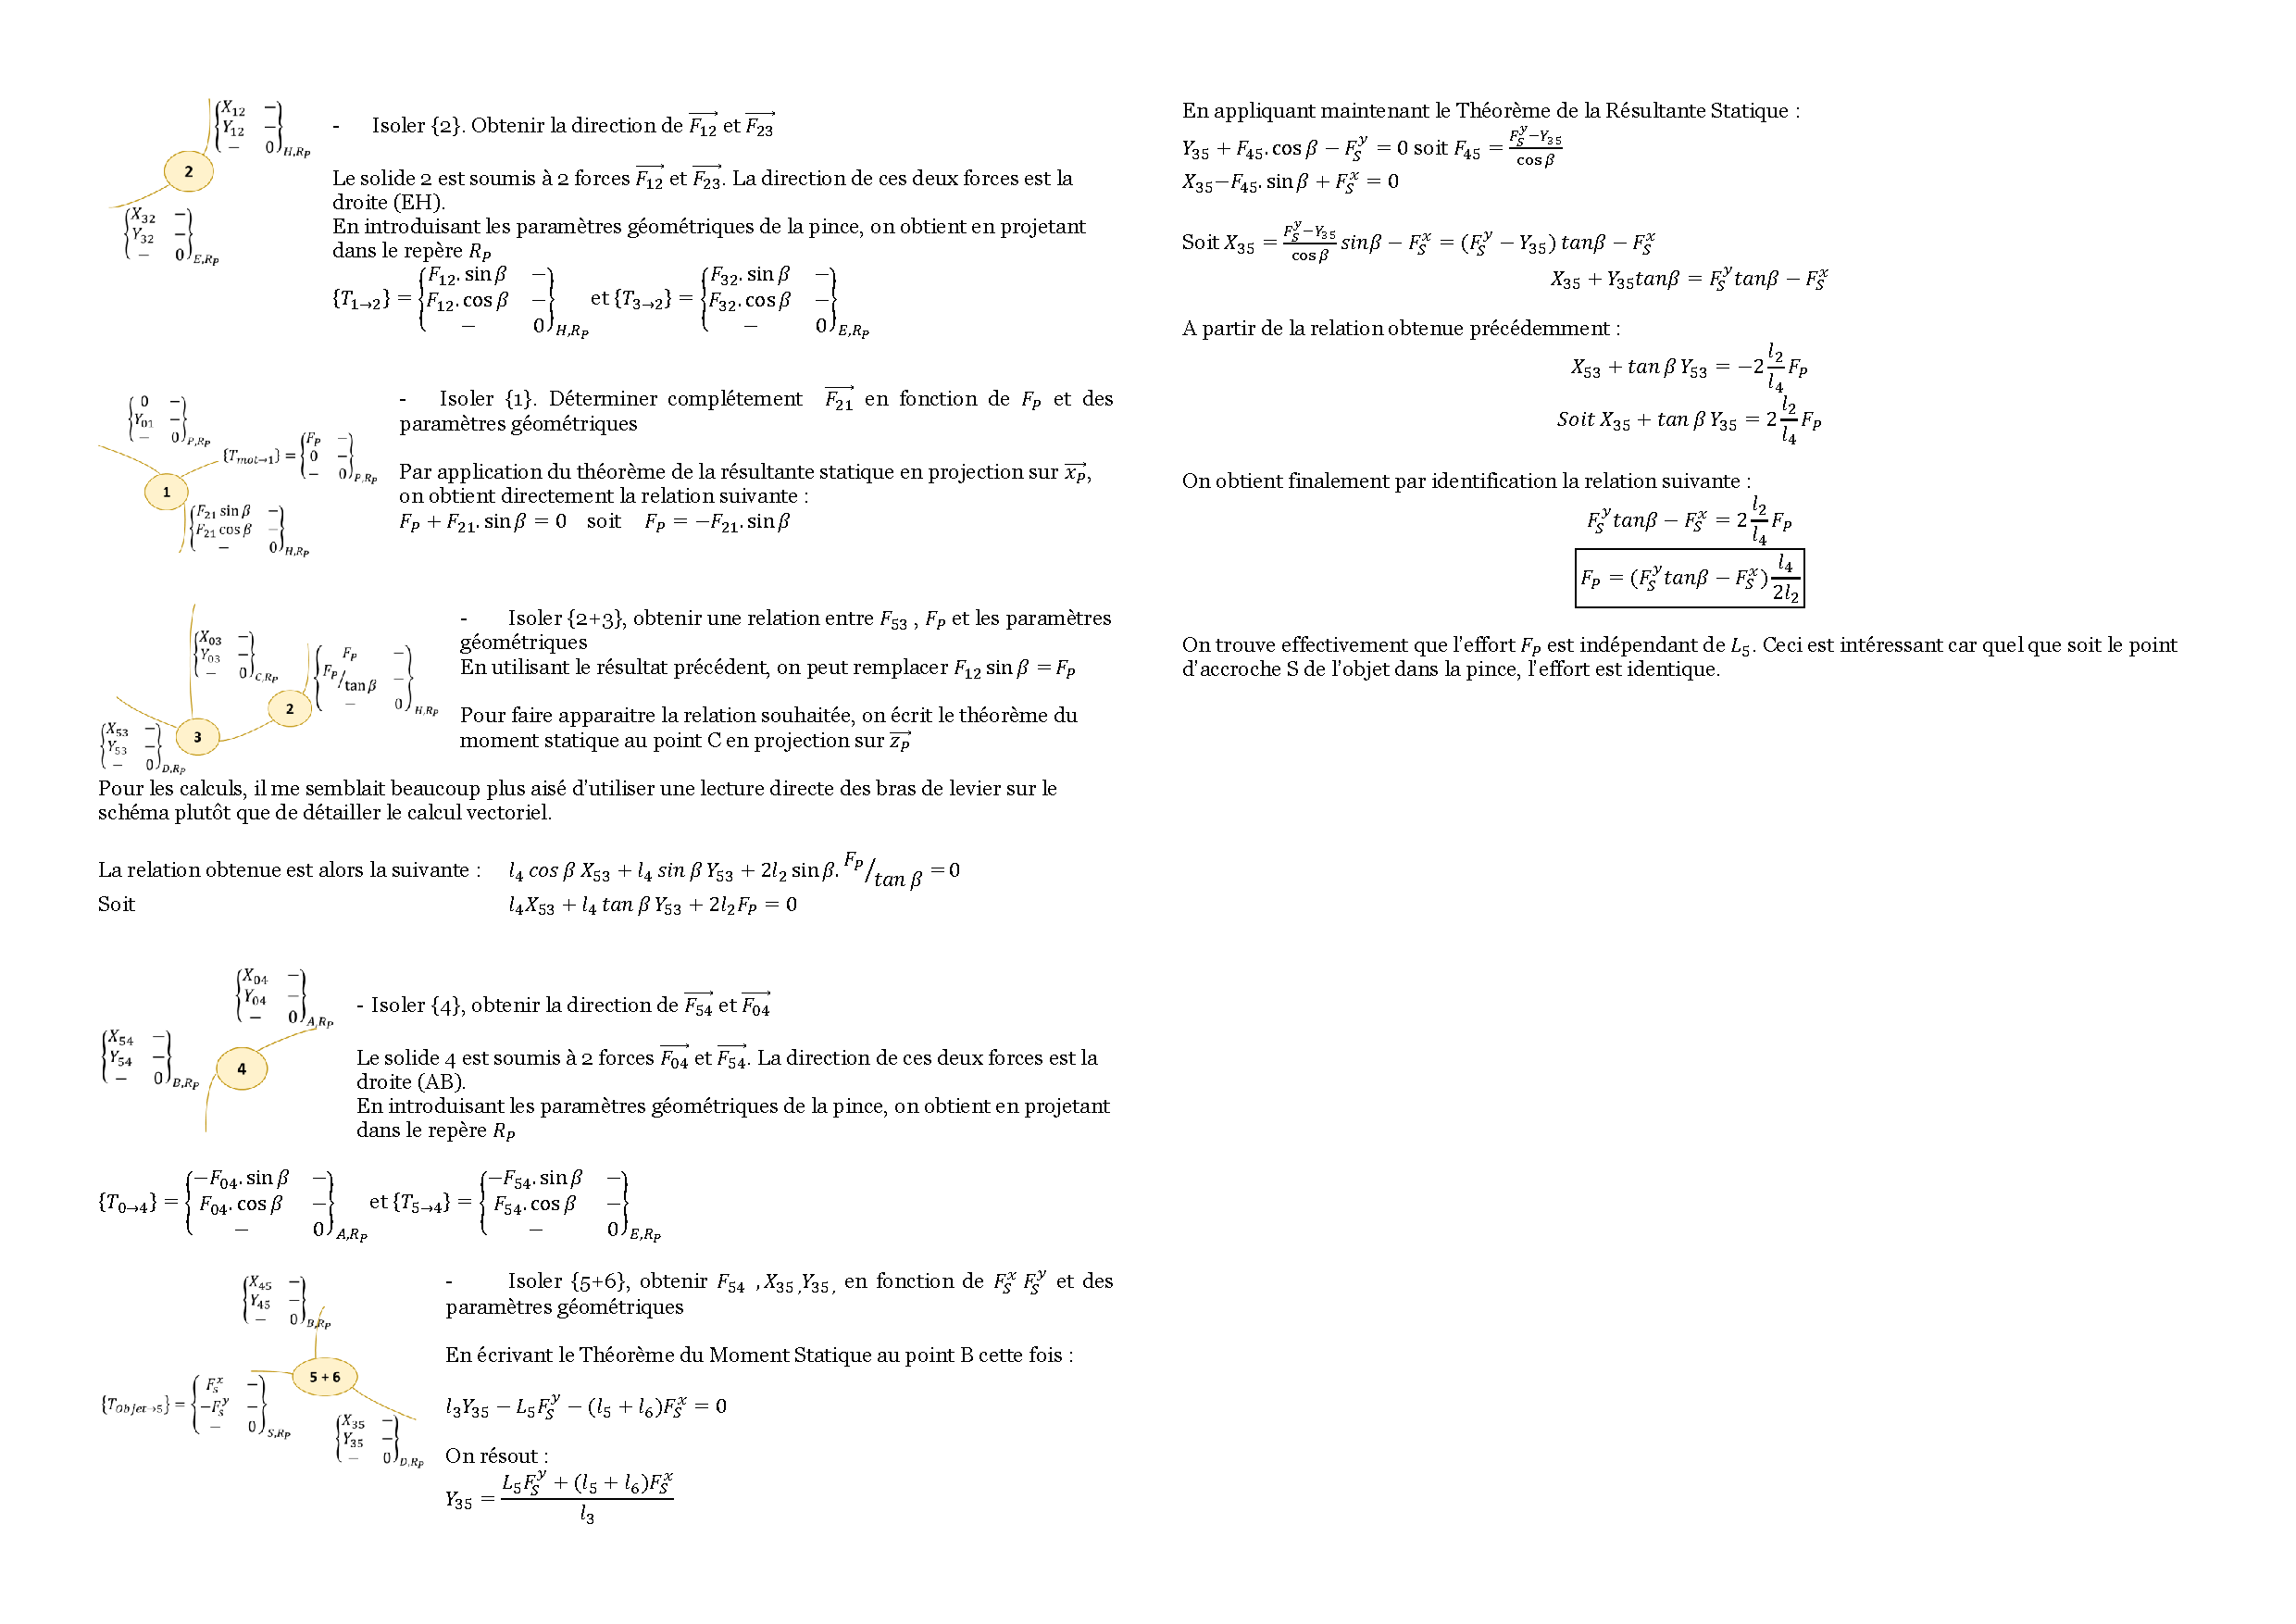
\includegraphics[width=\linewidth]{PFS}}
\end{figure}

\end{corrige}
\else
\fi

\ifprof
\else
On représente sur la \autoref{fig_24}  l'évolution de $\tan \beta$ en fonction du rayon $R$ de l'objet à saisir sur la plage $R =[\SI{20}{mm}, \SI{165}{mm}]$.

\begin{figure}[H]
\centering
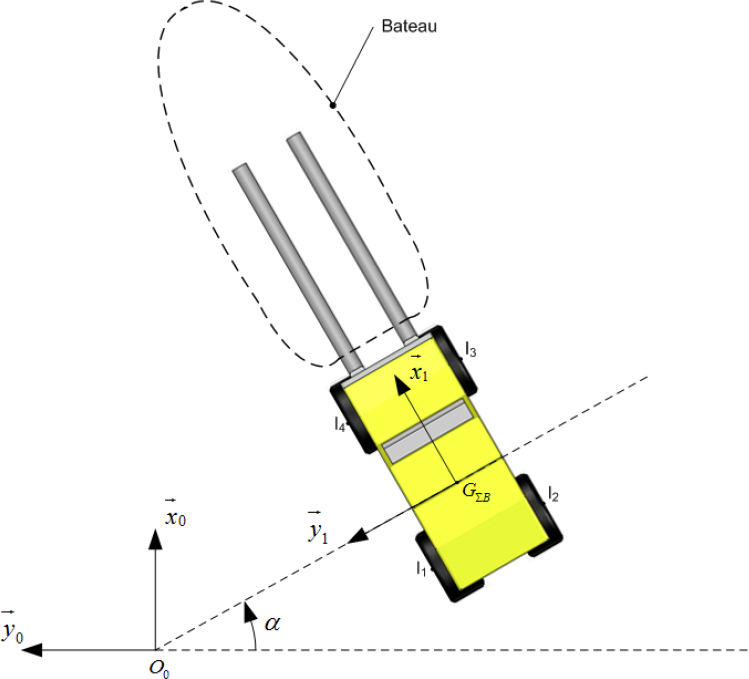
\includegraphics[width=10cm]{fig_24.png}
\caption{Evolution de $\tan \beta$ en fonction de $R$ \label{fig_24}}
\end{figure}
\fi


%Q5.6 : 
\question{Commenter ce graphe, en particulier pour les valeurs extrêmes du rayon $R$.}
\ifprof
\begin{corrige}
On remarque que :
\begin{itemize}
\item quand $R$ est grand, l’effort $F_P$est quasi-indépendant de l’effort normal $F_S^y$ de la pince sur l’objet. 
\item quand $R$ est petit, l’effort $F_P$ dépend quasi-uniquement de l’effort normal $F_S^y$. La capacité de préhension est fortement diminuée pour des petits rayons.
\end{itemize}
\end{corrige}
\else
\fi

%Q5.7 : 
\question{En supposant un modèle de frottement de Coulomb (le coefficient de frottement est noté $f$), 
montrer que l'objet peut être saisi et soulevé sans aucune action de poussée $F_p$ du moteur
lorsque le rayon de l'objet est tel que $R \geq R_{\text{min}}$. On précisera l'expression de $ R_{\text{min}}$ , on donnera sa
valeur pour $f =2$, et on commentera ce caractère particulier de la pince en donnant un avantage
et un inconvénient.}
\ifprof
\begin{corrige}
En supposant un modèle de frottement de Coulomb, on a à la limite de l'adhérence (action de l’objet 6 sur le cône de frottement)
$|F_S^x |=f |F_S^y |$. L’effort $F_P$ est nul lorsque $\tan\beta =f$.
Dans ces conditions, le rayon 
$
R=R_{\text{min}} = d+l_4 \sin \left (\tan^{-1} f \right) -l_5 -l_6$.

\end{corrige}
\else
\fi

%Q5.8 : 
\question{Pour $R < R_{\text{min}}$, donner la relation entre l'effort de poussée $F_p$ et la masse $m_{\text{objet}}$ de l'objet
à saisir, ainsi qu'entre l'effort de poussée $F_p$ et l'effort de serrage$F_S^y$ . En déduire la valeur de
l'effort de poussée maximal à fournir pour respecter le cahier des charges avec $f =2$.}
\ifprof
\begin{corrige}
Dans le cas où $R<R_{\text{min}}$ on a :
$F_P=\left(\dfrac{m_{\text{objet}}g}{3} \tan \beta -f \dfrac{m_{\text{objet}} g}{3}\right) \dfrac{l_4}{2l_2}$ 

Le cahier des charges impose  $R_{\text{min}}=0,04$ soit  $\tan\beta =6$ d’après la figure 24 et  $m_{\text{maxi}}=\SI{2,5}{kg}$

Dans ces conditions,
$F_P=\left(\dfrac{2,5\times 10}{3} \times 6- \dfrac{2 \times 2,5\times 10}{3}\right)  \dfrac{3}{4}=\SI{25}{N}$.

Pour les trois doigts, l’effort sera donc de \SI{75}{N}.

\end{corrige}
\else
\fi

\subsection{Asservissement de l'effort}

\begin{obj}
Dans cette sous-partie, on étudie l’asservissement en effort de la pince. En lien avec la
sous-partie précédente, on se place dans la configuration $R < R_{\text{min}}$ et on donne la relation
$F_s^y = K_{\beta} F_p$.
\end{obj}

\ifprof
\else
La pince a un capteur d'effort pour mesurer et contrôler la force de serrage. Pour l'asservissement
de la pince, une régulation en effort est faite. Le schéma blocs de la \autoref{fig_25} présente la structure
de contrôle de la pince.


\begin{figure}[H]
\centering
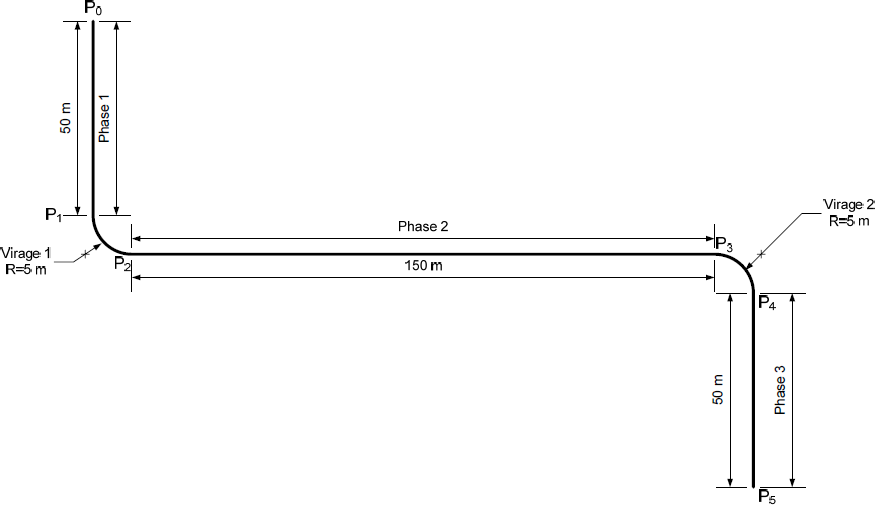
\includegraphics[width=.9\linewidth]{fig_25.png}
\caption{Schéma d'asservissement \label{fig_25}}
\end{figure}

\fi

%Q5.9 : 
\question{Quel est l'intérêt pratique de la régulation mise en place ?}
\ifprof
\begin{corrige}
La régulation en place permet de contrôler l’effort normal et donc de contrôler le non-glissement de l’objet par rapport à la pince.
\end{corrige}
\else
\fi
Pour l’étude en asservissement de la pince, on fixe $K_{\beta} = 2,2$.
On donne les caractéristiques du système suivantes.

\ifprof
\else
\begin{table}[H]
\centering
\begin{tabular}{lll}
\hline
$R$ &  résistance d'induit 		& $\SI{7,2}{\Omega}$ \\ \hline
$L$ &   inductance d'induit 	& \SI{2,56}{mH} \\ \hline
$K_t$ &  constante de couple 	& \SI{0,82}{Nm/A} \\ \hline
$K_e$ &  constante de fcem 	& \SI{86}{V/1000tr/min} \\ \hline
$J_{\text{eq}}$ &  moment d'inertie 	& \SI{3,45e-4}{ kg m^2} \\ \hline
$Kr$ &  rapport du réducteur 	& $54/33=1,636$ \\ \hline
$K_{\text{ve}}$ & pas du système vis-écrou & $\SI{4}{mm}$  \\ \hline
\end{tabular}
\end{table}
\fi


%Q5.10 : 
\question{En considérant $P_F=0$ (perturbation nulle) et $L=0$ (inductance nulle), calculer la fonction de transfert
$\dfrac{F_S^y}{F_c}$ et la mettre sous la forme canonique $\dfrac{K}{1+Ap+Bp^2}$. Identifier les paramètres $K$,
$A$ et $B$.}
\ifprof
\begin{corrige}

$\dfrac{F_S^y (p)}{F_C (p)}=\dfrac{C_f K_t K_r K_{ve} K_{\beta}}{R+C_f K_t K_r K_{ve} K_{\beta} } \times \dfrac{1}{1+\dfrac{K_e K_t}{R+C_f K_t K_r K_{ve} K_{\beta} }p+\dfrac{RJ_{eq}}{R+C_f K_t K_r K_{ve} K_{\beta} } p^2}$.


Par identification, on obtient :
$K=\dfrac{C_f K_t K_r K_{ve} K_{\beta}}{R+C_f K_t K_r K_{ve} K_{\beta}}$
$A=\dfrac{K_e K_t}{R+C_f K_t K_r K_{ve} K_{\beta} }$;
$B=\dfrac{RJ_{\text{eq}}}{R+C_f K_t K_r K_ve K_{\beta} }$.

\end{corrige}
\else
\fi

On souhaite une erreur de position inférieure à 1\%.

%Q5.11 : 
\question{Calculer la valeur de $C_f$ permettant de respecter cette contrainte.}
\ifprof
\begin{corrige}
L’erreur statique $\varepsilon_p$ pour une entrée en échelon d’amplitude $F_{\text{c0}}$ vaut :

$\varepsilon_p=(1-K) F_{\text{c0}}=\dfrac{R}{R+C_f K_t K_r K_{ve} K_{\beta} } F_{\text{c0}}$.

Pour obtenir une erreur inférieure à 1\%, il faut :
$C_f>\dfrac{0,99R}{0,01K_t K_r K_{ve} K_{\beta} } \simeq 60370$.

\end{corrige}
\else
\fi

%Q5.12: 
\question{Bien qu’il y ait un intégrateur dans la chaîne directe, indiquer pourquoi l’erreur statique est non-nulle.}
\ifprof
\begin{corrige}
L’intégrateur est placé  après la perturbation (modélisée comme un couple résistant sur le moteur). L’erreur ne peut donc être nulle malgré la présence de l’intégrateur (il y a une perturbation inhérente à l’effort $F_S^y$).
On peut aussi dire que la FTBO est de classe 0 (on ne retrouve pas l’intégrateur pur dans l’écriture de la FTBO).

\end{corrige}
\else
\fi

%Q5.13: 
\question{En considérant une valeur du correcteur permettant de valider le critère d’erreur de
position, ce critère sera-t-il toujours validé si on ne néglige plus les perturbations ? Comment le
démontrer ?}
\ifprof
\begin{corrige}
La perturbation agissant sur la valeur de l’erreur globale, en l’absence d’intégrateur pur en amont de la perturbation, le critère ne sera plus systématiquement validé. On peut le démontrer par le Théorème de la valeur Finale par exemple.
\end{corrige}
\else
\fi

%Q5.14: 
\question{Le coefficient  $K_{\beta}$ a-t-il une influence sur l’asservissement ? Pourquoi ne peut-on pas
considérer $K_{\beta}$ comme une constante ?}
\ifprof
\begin{corrige}
Le coefficient $K_{\beta}$ représente la loi entrée-sortie du mécanisme reliant la position linéaire du vérin et la position de la pince. Cette relation est non-linéaire car elle fait intervenir des fonctions trigonométriques de l’angle ${\beta}$. Bien évidemment, ce coefficient a une influence sur le comportement de l’asservissement et un choix sera fait sur la zone de fonctionnement qui sera linéarisée.
\end{corrige}
\else
\fi

Pour des raisons techniques, il n'est pas possible d'utiliser un capteur d'effort en bout de pince.

%Q5.15 : 
\question{Est-il techniquement possible d'asservir le système sans ce capteur d'effort ? Expliquer le
raisonnement.}
\ifprof
\begin{corrige}
Bien qu’il ne soit pas possible de positionner un capteur d’effort, il est possible d’asservir cette grandeur. En effet, il est possible de trouver une grandeur image de l’effort normal par le biais par exemple de la mesure du courant électrique circulant dans l’induit du moteur. Ce courant est une image du couple moteur qui sera lui-même image de l’effort normal. Dans ce contexte, la relation non-linéaire du mécanisme sera une difficulté supplémentaire à surmonter si la mesure est indirecte.
\end{corrige}
\else
\fi
\ifprof
\else
Dans l'étude précédente, la masse de l'objet et le coefficient de frottement entre la pince et l'objet
sont supposés connus. Cependant, ce n’est pas le cas en pratique et il peut en résulter un
glissement possible de l’objet si ces paramètres sont mal évalués.
\fi

%Q5.16 : 
\question{Quel moyen peut-on imaginer afin de limiter le glissement de l’objet ? Expliquer le
raisonnement.}
\ifprof
\begin{corrige}
Afin de limiter le glissement, il faut :
\begin{itemize}
\item augmenter l’effort normal (et maitriser également le rayon de la pièce soulevée);
\item jouer sur le couple de matériaux en contact afin de maximiser le coefficient d’adhérence.
\end{itemize}

\end{corrige}
\else
\fi

